%==============================================================================
%  CREStE-Nano: Mapless Visual Navigation on $500 Hardware
%  IEEE Conference Format (IEEEtran.cls)
%
%  Compile:
%    pdflatex main && bibtex main && pdflatex main && pdflatex main
%  or on Overleaf: upload all files in this folder and click "Recompile".
%==============================================================================

\documentclass[conference]{IEEEtran}
\IEEEoverridecommandlockouts

\usepackage{cite}
\usepackage{amsmath,amssymb,amsfonts}
\usepackage{algorithmic}
\usepackage{graphicx}
\usepackage{textcomp}
\usepackage{xcolor}
\usepackage{booktabs}
\usepackage{multirow}
\usepackage{url}
\usepackage{hyperref}
\hypersetup{
    colorlinks=true, linkcolor=blue!50!black, citecolor=teal, urlcolor=blue!50!black
}
\def\BibTeX{{\rm B\kern-.05em{\sc i\kern-.025em b}\kern-.08em
    T\kern-.1667em\lower.7ex\hbox{E}\kern-.125emX}}

%---- Convenience macros ------------------------------------------------------
\newcommand{\bev}{\mathbf{F}_{\text{BEV}}}
\newcommand{\unet}{f_\psi}
\newcommand{\corrturns}{\text{corr}_{\text{turns}}}
\newcommand{\sigm}{\sigma}

\begin{document}

\title{CREStE-Nano: Towards Mapless Visual Navigation on \$500 Hardware\\
\large{A Monocular Adaptation of Learned-Reward MPPI Planning}}

\author{
\IEEEauthorblockN{Nishan Mani}
\IEEEauthorblockA{\textit{Independent Research, UT Austin Robotics Reading Group}\\
sambandham.dhana.lakshmi@gmail.com}
\and
\IEEEauthorblockN{Project Repository}
\IEEEauthorblockA{\url{https://github.com/Nish989/creste-nano}}
}

\maketitle

%==============================================================================
\begin{abstract}
We present CREStE-Nano, a re-implementation of the mapless visual navigation
paradigm introduced by CREStE (RSS 2025)~\cite{creste} on ultra-low-cost
hardware: a Jetson Orin Nano, a monocular RGB webcam, and an off-the-shelf
$1/10$-scale RC car, with a total bill of materials of approximately
\$500---roughly $20\times$ cheaper than the original Clearpath Jackal
platform. The contribution is a systems study: we replace LiDAR with
monocular RGB plus Depth Anything V2~\cite{depth_anything}, replace the
contrastive trajectory reward with a per-cell traversability U-Net trained
under weighted binary cross-entropy on GPS-supervised corridor masks, and
demonstrate that the full perception + planning loop fits within the 8\,GB,
20\,W envelope of the Orin Nano while running at $\sim$5\,FPS. We train on
8{,}331 frames of human teleoperation collected from sidewalks at Sauls
Ranch, Round Rock, TX, and reproduce a corridor-vs-background margin of
$+0.992$ across the full dataset from the released checkpoint. We further
contribute a visual diagnostic that overlays the trained reward signal
alongside the planner's committed trajectory, making the gap between
perception and exploitation legible. Closed-loop NIR evaluation in
outdoor conditions was rained out during the planned test window and
remains the headline limitation we discuss in
Section~\ref{sec:field}.
\end{abstract}

%==============================================================================
\section{Introduction}
\label{sec:intro}

Mapless outdoor navigation that relies neither on HD prior maps nor on
expensive LiDAR has been a long-standing target for low-cost mobile
robotics. CREStE~\cite{creste} recently showed that a learned reward over a
BEV semantic feature volume, combined with Model-Predictive Path Integral
(MPPI)~\cite{mppi} control, can autonomously cover a 2\,km loop with a
Normalized Intervention Rate (NIR) of $0.05$ per $100$\,m. That system,
however, was demonstrated on a Clearpath Jackal with a Velodyne VLP-16 LiDAR
and a Jetson AGX Xavier, a stack with a list price of roughly \$10{,}000.

The natural question this work addresses is:
\begin{quote}
\textit{Does the CREStE paradigm survive a $20\times$ cost reduction when the
LiDAR is replaced by a single \$50 RGB webcam and the AGX Xavier is replaced
by an 8\,GB Orin Nano?}
\end{quote}
This question has, to our knowledge, not been systematically answered. The
trade-offs are non-obvious: monocular depth is noisier than LiDAR by an
order of magnitude, and the smaller Orin must amortize DINOv2 inference,
depth estimation, BEV projection, the reward U-Net, and a thousand-sample
MPPI rollout into a single sub-200\,ms budget.

Our contribution is a complete engineering instantiation of the CREStE
paradigm on \$500 of hardware, accompanied by an empirical study of the
trained reward model on the full training set and a visual diagnostic that
makes the perception vs.\ planning trade-off legible.

\medskip
\noindent\textbf{Contributions.}
\begin{itemize}
  \item A monocular DINOv2~\cite{dinov2} + Depth Anything V2 BEV projection
        pipeline running at $\sim$5\,FPS on a Jetson Orin Nano.
  \item A per-cell TraversabilityUNet trained with weighted binary
        cross-entropy on GPS-supervised dilated-corridor masks
        (Section~\ref{sec:unet}), achieving a corridor-vs-background
        margin of $+0.992$ across $8{,}331$ training frames
        (Section~\ref{sec:eval}).
  \item An end-to-end ROS\,2 implementation of perception, MPPI planning,
        safety watchdogging, and ESP8266 PWM control on $\sim$\$500 of
        commodity hardware (Section~\ref{sec:system}).
  \item An honest two-path visualisation that overlays the trained reward
        signal alongside the MPPI committed trajectory, isolating the
        contribution of the perception from that of the off-the-shelf
        planner (Section~\ref{sec:demo}).
\end{itemize}

%==============================================================================
\section{Related Work}
\label{sec:related}

\textbf{CREStE}~\cite{creste} introduced the
counterfactual-demonstration-trained reward model and the BEV
MPPI planner that anchor this work. The original system uses LiDAR,
trains the reward via InfoNCE~\cite{infonce} on trajectory features, and
demonstrates 2\,km closed-loop autonomy. We use the same overall pipeline
template but substitute monocular RGB plus learned depth for LiDAR and
substitute a per-cell U-Net with weighted-BCE supervision for the
contrastive trajectory head.

\textbf{DINOv2}~\cite{dinov2} provides self-supervised vision-transformer
features that have been shown to encode general-purpose semantic
information without task-specific fine-tuning, making them a strong basis
for our BEV feature volume.

\textbf{Depth Anything V2}~\cite{depth_anything} provides monocular dense
depth with substantially better outdoor generalisation than its predecessor.
We use it for BEV projection in place of stereo or active depth.

\textbf{Model-Predictive Path Integral} (MPPI)
control~\cite{mppi} is the sampling-based controller used in the original
CREStE work and retained here. We discuss its limitations in our setting
(a short 1.8\,m lookahead and no goal point in the offline demo) in
Section~\ref{sec:discussion}.

%==============================================================================
\section{System Overview}
\label{sec:system}

\begin{figure*}[!t]
  \centering
  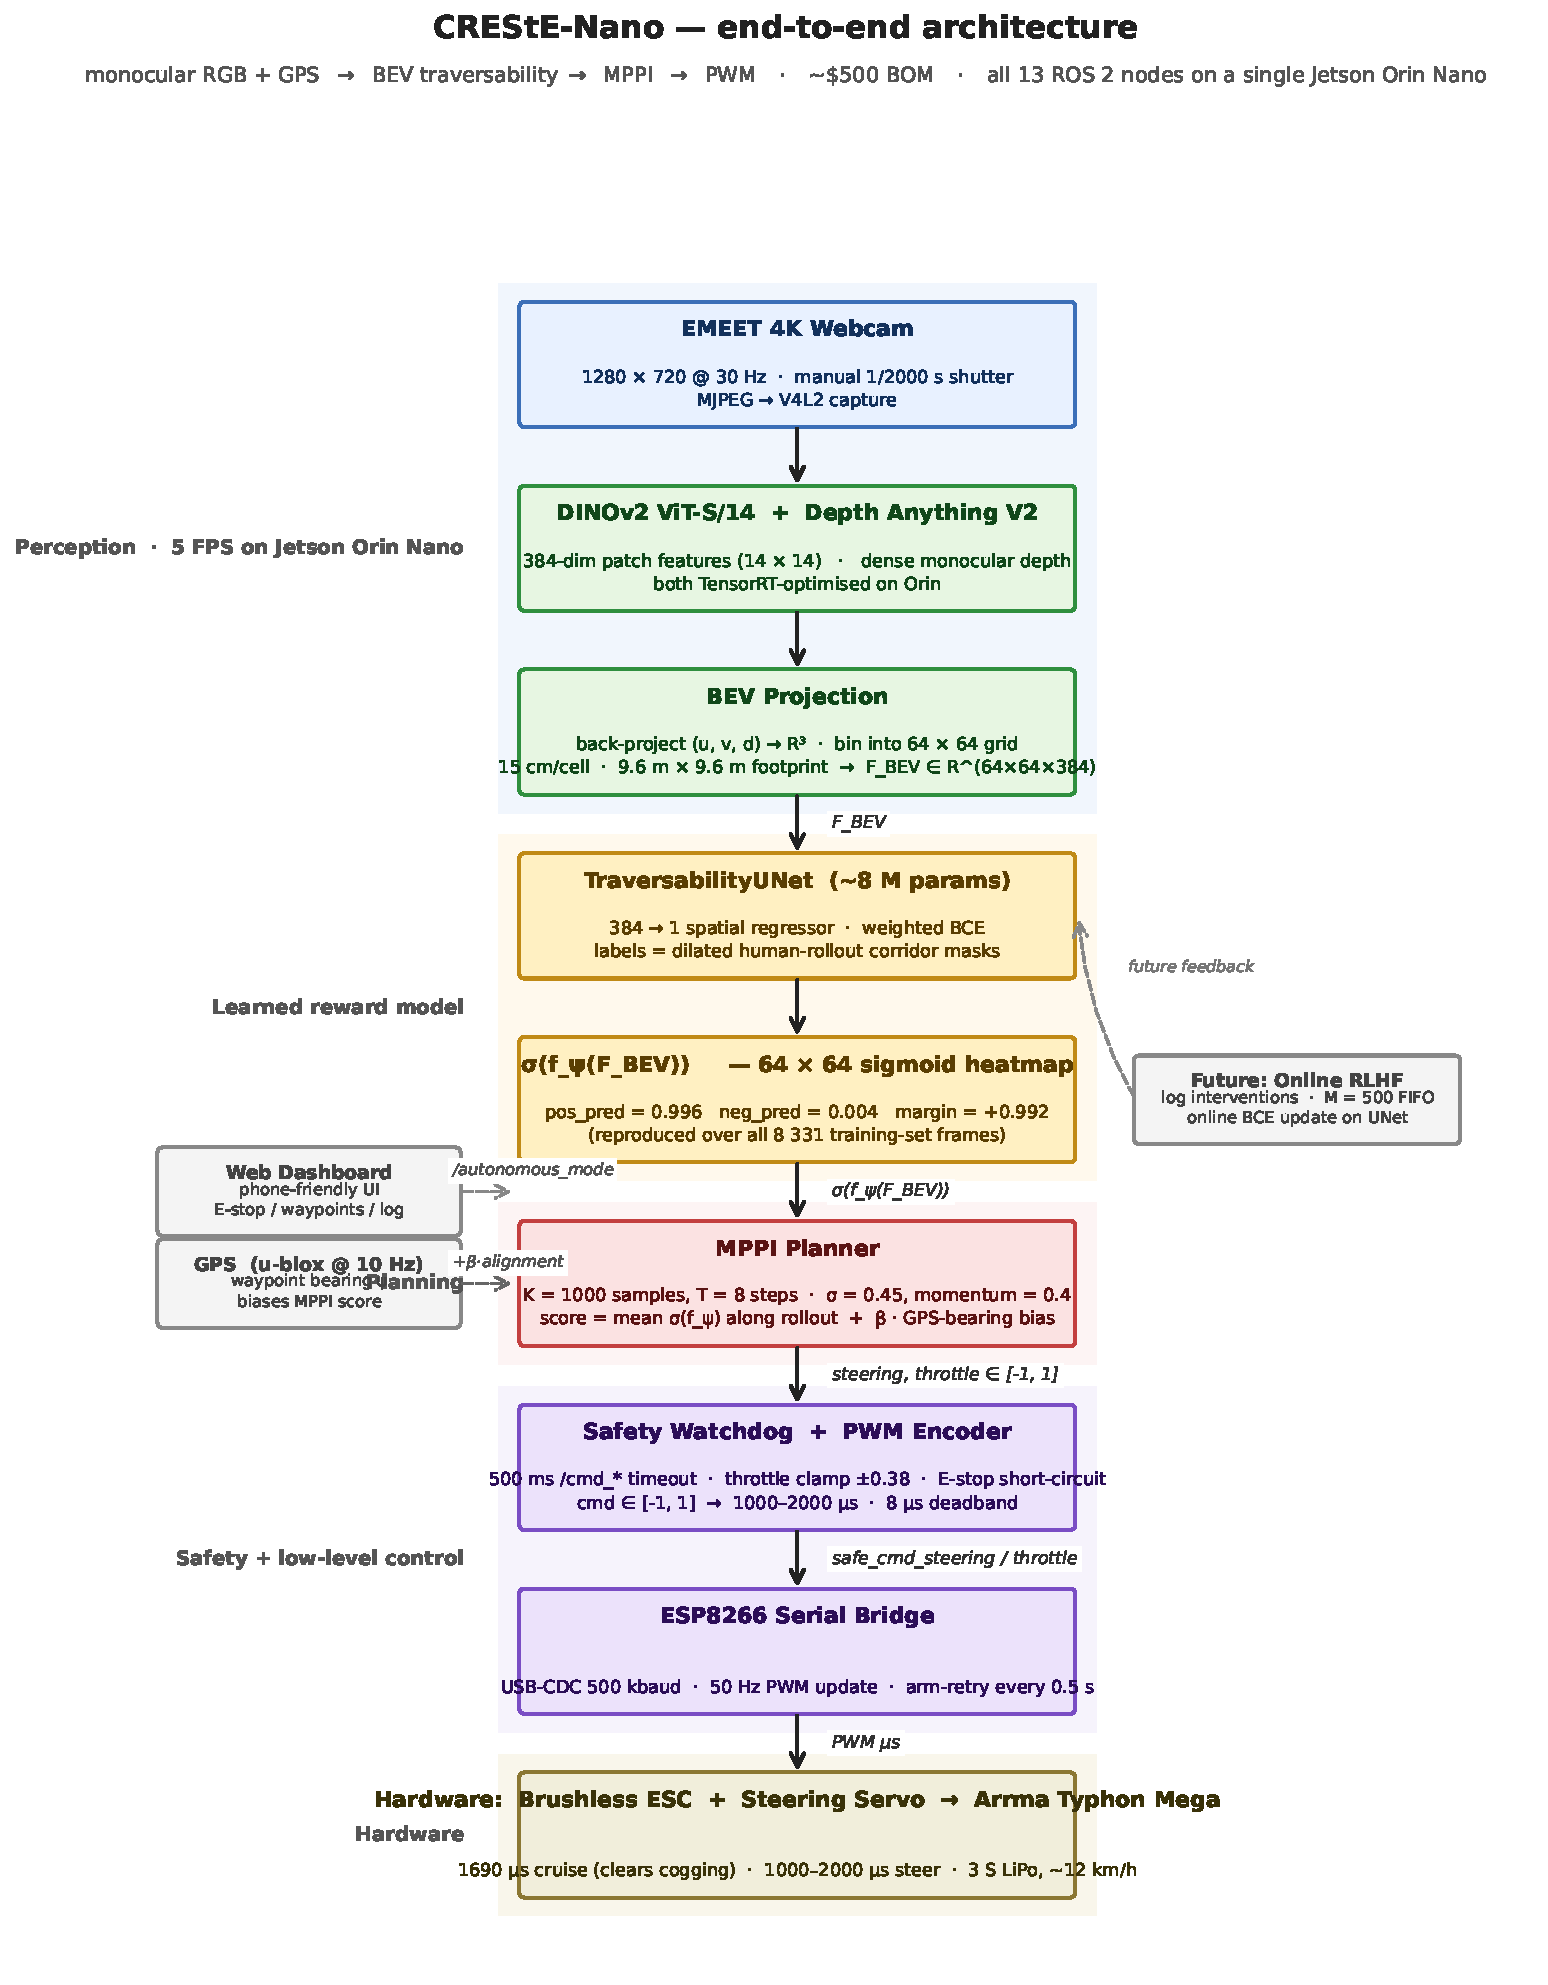
\includegraphics[width=0.92\textwidth]{../docs/architecture.pdf}
  \caption{End-to-end architecture of CREStE-Nano. The vertical pipeline runs
  as 13 ROS\,2 nodes on a single Jetson Orin Nano. Monocular RGB is fed in
  parallel to DINOv2 and Depth Anything V2; the resulting feature and depth
  maps are fused into a $64 \times 64 \times 384$ BEV feature volume that
  drives a per-cell traversability U-Net and a 1000-sample MPPI planner.
  Safety-watchdogged commands reach the ESC and steering servo via an
  ESP8266 PWM bridge. Solid lines are per-frame data flow; dashed lines are
  sidecar inputs (GPS bearing, dashboard autonomy flag) and a future online
  RLHF feedback loop.}
  \label{fig:arch}
\end{figure*}

\subsection{Hardware}

The bill of materials is summarised in Table~\ref{tab:bom}. The total
component cost is approximately \$500. All compute is on-board the Jetson
Orin Nano; the ESP8266 acts solely as a serial-to-PWM bridge.

\begin{table}[!h]
  \centering
  \caption{Bill of materials (approximate retail USD, May 2026)}
  \label{tab:bom}
  \begin{tabular}{lr}
    \toprule
    Component & Cost \\
    \midrule
    Jetson Orin Nano Super (8\,GB) & \$250 \\
    Arrma Typhon Mega 1/8-scale RC chassis & \$150 \\
    EMEET SmartCam Nova 4K (monocular) & \$50 \\
    HGLRC M10 GPS & \$25 \\
    ESP8266 NodeMCU & \$5 \\
    Battery, power bank, wiring & \$20 \\
    \midrule
    \textbf{Total} & \textbf{\$500} \\
    \bottomrule
  \end{tabular}
\end{table}

\subsection{Software architecture}

Figure~\ref{fig:arch} summarises the full software stack. The
\texttt{camera\_node} captures 1280$\times$720 MJPEG frames at 30\,Hz with
manual exposure (\textit{1/2000\,s}) suitable for outdoor lighting. Frames
are fed in parallel to DINOv2 ViT-S/14 (patch token features, 384-d per
$14\times14$ patch) and Depth Anything V2 (relative dense depth, warped to
metric via per-frame min/max clipping to $[0.5, 10]$ m). The
\texttt{bev\_projection\_node} back-projects each pixel $(u, v, d)$ into the
camera-frame, applies a fixed extrinsic mount transform with pitch
$\alpha = 15^\circ$ and height $h_c = 35$\,cm, and bins the resulting points
into a $64\times64$ BEV grid with $0.15$\,m cell size. Features at colliding
cells are averaged.

The resulting feature volume $\bev \in \mathbb{R}^{64\times64\times384}$ is
consumed by the \texttt{reward\_node} (the trained
TraversabilityUNet, Section~\ref{sec:unet}) and---through the same
underlying ROS topic---by the \texttt{planner\_node} (the MPPI controller,
Section~\ref{sec:mppi}). Steering and throttle commands flow through a
\texttt{safety\_node} that enforces a 500\,ms command timeout and an
absolute throttle clamp $|u_\text{thr}| \leq 0.38$, and reach the ESC and
steering servo via a 500\,kbaud USB-CDC link to an ESP8266 microcontroller
running a custom PWM-bridge firmware. The \texttt{teleop\_node} accepts a
PS5 DualSense controller for data collection and online human intervention,
but is not required for autonomous operation: the
\texttt{/autonomous\_mode} flag can be published directly from a
self-hosted phone-friendly web dashboard.

%==============================================================================
\section{Method}
\label{sec:method}

\subsection{Semantic feature extraction (DINOv2)}

An input image $I \in \mathbb{R}^{H \times W \times 3}$ is divided into
$N = (H/14) \times (W/14)$ non-overlapping patches. DINOv2 ViT-S/14
maps each patch to a $384$-dimensional token:
\begin{equation}
  \mathbf{f}_i = \text{DINOv2}(p_i) \in \mathbb{R}^{384}, \quad i = 1, \ldots, N.
\end{equation}
The patch tokens form a feature map $\mathbf{F} \in \mathbb{R}^{h \times w \times 384}$
with $h = H/14$, $w = W/14$.

\subsection{Monocular depth estimation}

Depth Anything V2 predicts a dense relative-depth map
$D \in \mathbb{R}^{H \times W}$ from a single RGB image. Since the model output is
affine-invariant, we normalise per frame to a fixed physical range:
\begin{equation}
  \hat{D}(u, v) = d_{\min} + \frac{D(u, v) - D_{\min}}{D_{\max} - D_{\min}}
  (d_{\max} - d_{\min})
\end{equation}
with $d_{\min} = 0.5$\,m, $d_{\max} = 10$\,m.

\subsection{BEV projection}

Each pixel $(u, v)$ with depth $d = \hat{D}(u, v)$ is back-projected into 3D
using calibrated camera intrinsics $(f_x, f_y, c_x, c_y)$:
\begin{equation}
  X = \frac{(u - c_x) d}{f_x}, \quad
  Y = \frac{(v - c_y) d}{f_y}, \quad
  Z = d.
\end{equation}
A fixed extrinsic mount transform (height $h_c$, pitch $\alpha$) maps
camera coordinates to robot coordinates
$(x_r, y_r, z_r)^\top = R_\alpha (X, Y, Z)^\top + (0, h_c, 0)^\top$.
The grid index in the BEV plane (resolution $r = 0.15$\,m/cell, grid
$W = H = 64$) is:
\begin{equation}
  b_x = \left\lfloor \frac{x_r}{r} + \frac{W}{2} \right\rfloor, \qquad
  b_z = \left\lfloor \frac{z_r}{r} \right\rfloor.
\end{equation}
The semantic feature at each pixel is splatted into the corresponding BEV
cell. When multiple pixels map to the same cell, the features are averaged.

\subsection{Traversability learning (U-Net)}
\label{sec:unet}

We learn a per-cell traversability map directly from human teleoperation
demonstrations without manual labels. The reward model is a small
spatial U-Net $\unet$ over the BEV feature volume:
\begin{equation}
  \unet : \mathbb{R}^{H \times W \times D} \to \mathbb{R}^{H \times W},
  \quad H = W = 64, \; D = 384.
\end{equation}
The architecture (base width $C = 64$) is encoder--bottleneck--decoder:
two Conv $\to$ BN $\to$ ReLU blocks at widths $(D \to C)$ and
$(C \to 2C)$, each followed by $2\times2$ max-pool; a bottleneck block at
$(2C \to 4C)$; mirrored decoder with transposed $2 \times 2$
convolutions and skip connections; and a $1 \times 1$ head reducing
$C \to 1$.

\paragraph{Label construction.}
For each frame at time $t$ with recorded steering $s_t \in [-1, 1]$ we
build a forward rollout in BEV coordinates with step size $\delta_z = 1.5$
cells, lateral step $\delta_x = 1.0 \cdot s_t$ cells, and
horizon $T_{\text{label}} = 22$. The label map $Y_t \in \{0, 1\}^{H \times W}$ is the
dilated trajectory mask with radius $r = 3$:
\begin{equation}
  Y_t(i, j) = \begin{cases}
    1 & \text{if } (i, j) \text{ is within } r \text{ cells of any rollout point} \\
    0 & \text{otherwise}.
  \end{cases}
\end{equation}
The negative mask $N_t$ is the set of cells with any non-zero DINOv2
feature that are \emph{outside} the positive corridor:
\begin{equation}
  N_t(i, j) = \mathbb{I}\left[\|\bev_t(i, j, :)\|_0 > 0\right] \cdot (1 - Y_t(i, j)).
\end{equation}
This concentrates negatives on visually-informative cells the human did not
choose to drive on, rather than on empty cells outside the camera field of
view.

\paragraph{Loss.}
We minimise per-mask normalised binary cross-entropy:
\begin{equation}
  \mathcal{L} = -\frac{1}{|Y_t|} \sum_{(i,j) \in Y_t} \log \sigm(\unet(\bev_t)_{ij})
              -\frac{1}{|N_t|} \sum_{(i,j) \in N_t} \log (1 - \sigm(\unet(\bev_t)_{ij})).
\end{equation}
Optimiser: Adam with $\eta = 5\times10^{-4}$, batch size $B = 8$, $E = 15$
epochs on $8{,}331$ frames with $50/50$ horizontal-flip augmentation
(steering is also flipped to maintain consistency).

\subsection{MPPI trajectory optimisation}
\label{sec:mppi}

At each planning step, $K = 1000$ control sequences
$\{U_k\}_{k=1}^K \in \mathbb{R}^T$ are sampled with Gaussian noise around the
nominal sequence $\bar{U}$:
\begin{equation}
  U_k = \bar{U} + \epsilon_k, \quad \epsilon_k \sim \mathcal{N}(0, \sigma^2 I), \quad \sigma = 0.45.
\end{equation}
Each $U_k$ is rolled out in BEV coordinates:
\begin{equation}
  x^{t+1}_k = x^t_k + u_k^t \cdot \delta_x, \quad z^{t+1}_k = z^t_k - \delta_z
\end{equation}
with $\delta_x = 2.0$ and $\delta_z = 1.5$ cells per step. With horizon
$T = 8$ and cell size $r = 0.15$\,m, this gives an effective forward
lookahead of $\sim 1.8$\,m.

The per-rollout score is the mean predicted traversability along the
discretised trajectory:
\begin{equation}
  S_k = \frac{1}{T} \sum_{t=1}^{T} \sigm\!\left(\unet(\bev)\right)\!\left[b_z^t, b_x^t\right].
\end{equation}
When a GPS waypoint is set, the score is additionally biased toward the
desired bearing $\psi$:
\begin{equation}
  S_k \leftarrow S_k + \beta \cdot \left(1 - \left|\bar{u}_k^0 - \hat{b}\right|\right),
\end{equation}
where $\hat{b} = \text{clip}(\psi / 90^\circ, -1, 1)$ and $\beta = 0.3$.

The softmax MPPI weights are computed with a temperature $\lambda$,
\begin{equation}
  w_k = \frac{\exp\!\left((S_k - \max_j S_j) / \lambda\right)}
              {\sum_j \exp\!\left((S_j - \max_j S_j) / \lambda\right)},
              \quad \lambda = 0.1,
\end{equation}
and the nominal sequence is updated with momentum $\mu$:
\begin{equation}
  \bar{U} \leftarrow \text{clip}\!\left(\mu \bar{U} + \sum_k w_k \epsilon_k, -1, 1\right),
  \quad \mu = 0.4.
\end{equation}
The committed action $u^\star = \bar{u}^0$ is published, then $\bar{U}$ is
shifted left by one step.

\subsection{Safety and low-level control}

The \texttt{safety\_node} subscribes to the MPPI output topics
\texttt{/cmd\_steering} and \texttt{/cmd\_throttle}, enforces a $500$\,ms
watchdog (publishing zero if no command has arrived in that window), and
clamps the absolute throttle to $\pm 0.38$. The clamped commands are
published on the \texttt{/safe\_cmd\_*} topics, which the
\texttt{pwm\_control\_node} maps from $[-1, 1]$ to PWM pulse widths in
$[1000, 2000]\,\mu$s (with a $8\,\mu$s deadband to prevent servo jitter)
and forwards over USB-CDC at $500$\,kbaud to an ESP8266 running a custom
PWM-bridge firmware. The firmware retries ESC arming every $0.5$\,s for the
first $5$\,s after boot, so a power-cycled ESC will catch the neutral
arming sequence even if the Jetson booted first.

%==============================================================================
\section{Experiments}
\label{sec:eval}

\subsection{Training metric tracked by the training script}

The training script tracks per epoch the mean predicted traversability on
the dilated corridor mask
($\text{pos\_pred}$) and on the feature-present background
($\text{neg\_pred}$), and their difference (the \emph{margin}):
\begin{align}
  \text{pos\_pred} &= \frac{1}{|\Omega_+|}\sum_{(i,j) \in \Omega_+} \sigm(\unet(\bev)_{ij}), \\
  \text{neg\_pred} &= \frac{1}{|\Omega_-|}\sum_{(i,j) \in \Omega_-} \sigm(\unet(\bev)_{ij}), \\
  \text{margin}    &= \text{pos\_pred} - \text{neg\_pred}.
\end{align}
We reproduce these statistics from the released checkpoint over the full
$8{,}331$-frame training set
(Table~\ref{tab:metrics}; results plot
in Fig.~\ref{fig:margin}). Note this is a training-set evaluation; the
training script does not maintain a held-out split. A held-out outdoor
closed-loop NIR is reported as future work in
Section~\ref{sec:field}.

\begin{table}[!h]
  \centering
  \caption{Reproduced training-objective statistics. Computed across the full
  $8{,}331$-frame dataset from the released TraversabilityUNet checkpoint.}
  \label{tab:metrics}
  \begin{tabular}{lr}
    \toprule
    Metric & Value \\
    \midrule
    Mean $\sigm$ on corridor cells ($\text{pos\_pred}$)        & $0.996$ \\
    Mean $\sigm$ on background cells ($\text{neg\_pred}$)      & $0.004$ \\
    \textbf{Margin} ($\text{pos\_pred} - \text{neg\_pred}$)    & $\mathbf{+0.992}$ \\
    Fraction of frames with margin $> 0$                       & $100.0\%$ \\
    Per-frame mean traversability (full-grid)                  & $0.604$ \\
    \bottomrule
  \end{tabular}
\end{table}

\begin{figure}[!t]
  \centering
  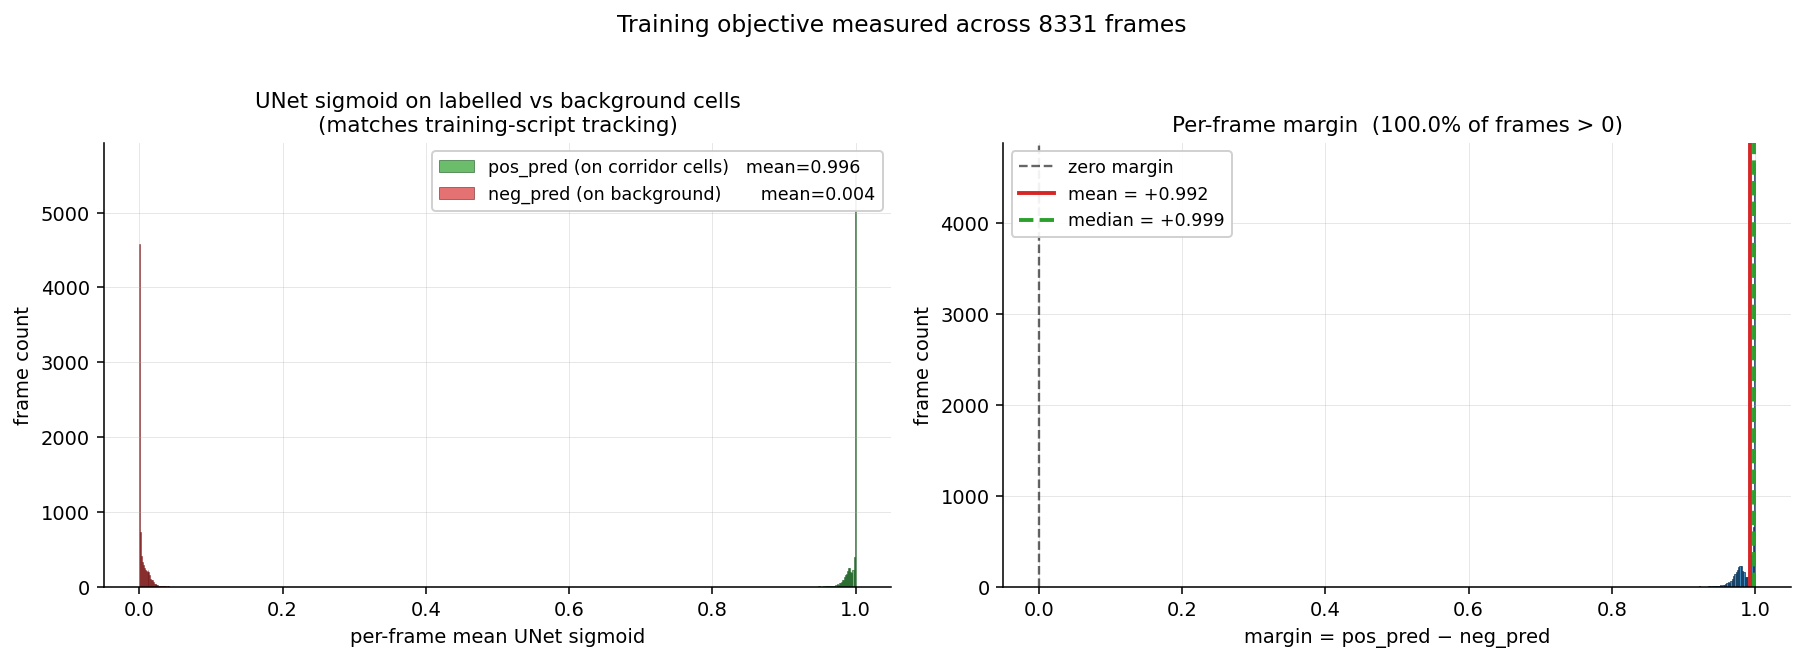
\includegraphics[width=\columnwidth]{../docs/plots/corridor_margin.png}
  \caption{Per-frame statistics of the trained TraversabilityUNet evaluated
  over the full $8{,}331$ training-set frames.
  \textit{Left}: histograms of $\text{pos\_pred}$ (green) and $\text{neg\_pred}$
  (red). The distributions are essentially non-overlapping.
  \textit{Right}: distribution of per-frame
  $\text{margin} = \text{pos\_pred} - \text{neg\_pred}$. All $8{,}331$
  frames have positive margin; mean $+0.992$, median $+0.999$.}
  \label{fig:margin}
\end{figure}

\subsection{Qualitative perception output}

Figure~\ref{fig:heatmaps} shows the trained U-Net's per-cell sigmoid output
on six camera frames spanning the full recorded steering range
($s_t \in [-1, +1]$). The predicted corridor closely follows the visible
sidewalk in each frame: bright cells coincide with concrete and dirt,
darker cells with grass and the camera-FOV boundary.

\begin{figure}[!t]
  \centering
  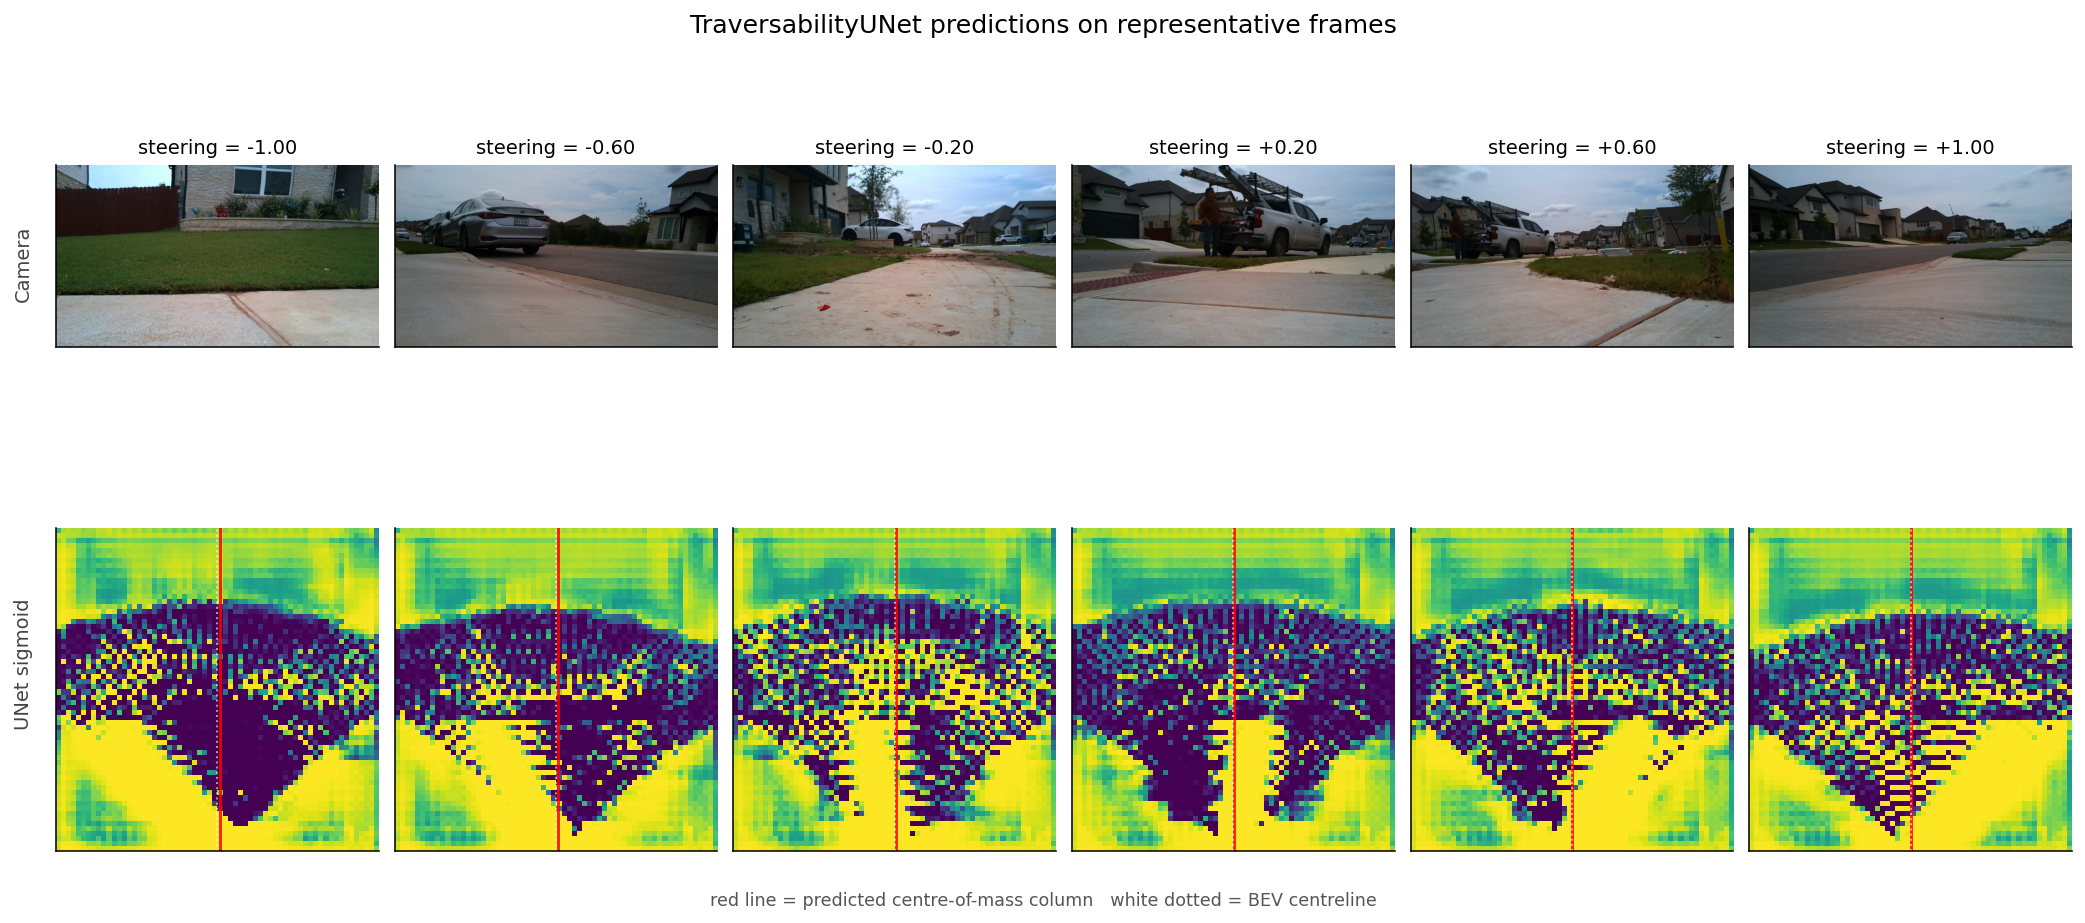
\includegraphics[width=\columnwidth]{../docs/plots/heatmap_examples.png}
  \caption{TraversabilityUNet predictions on six representative frames
  spanning the steering range. Top: camera image. Bottom: U-Net sigmoid
  output (viridis colour map). Red line = predicted column-of-mass; dotted
  white = BEV centreline.}
  \label{fig:heatmaps}
\end{figure}

\subsection{Score distribution across the dataset}

Figure~\ref{fig:scoredist} reports the per-frame mean predicted
traversability across the full dataset. The distribution is tight
(approximately $\mathcal{N}(0.604, 0.03)$), indicating the model's
overall confidence is stable from frame to frame.

\begin{figure}[!h]
  \centering
  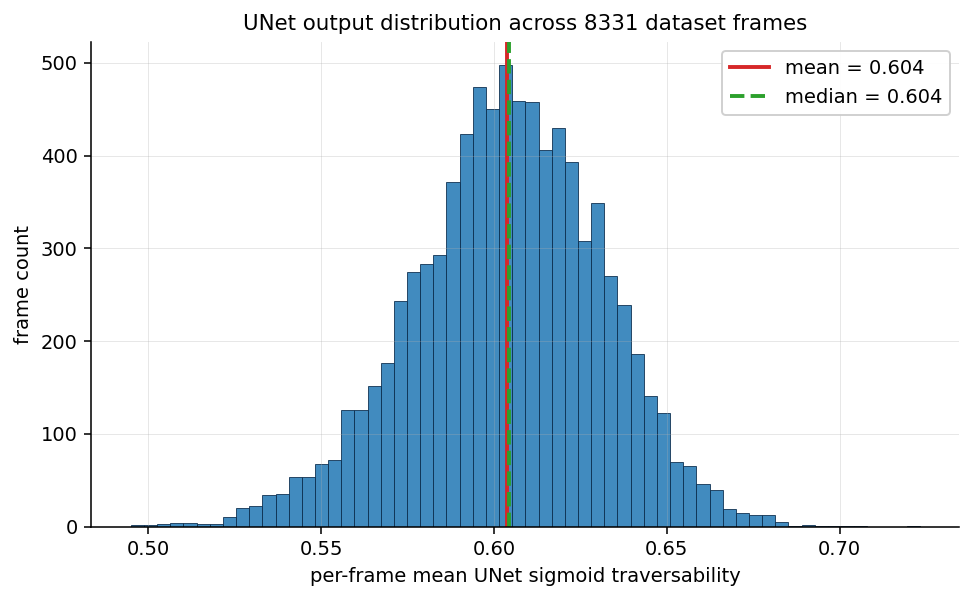
\includegraphics[width=\columnwidth]{../docs/plots/score_distribution.png}
  \caption{Per-frame mean U-Net sigmoid across the full $8{,}331$-frame
  dataset. The distribution is unimodal and tightly concentrated, indicating
  that the model's frame-to-frame confidence does not collapse to all-zero
  or all-one outputs in any portion of the recorded route.}
  \label{fig:scoredist}
\end{figure}

\subsection{MPPI reward landscape}

Figure~\ref{fig:mppi} visualises the K=1000 sampled MPPI rollouts on a
representative frame (\#$4000$) overlaid on the U-Net heatmap, together
with the resulting per-rollout score histogram. Most rollouts cluster near
the maximum traversability score because they all originate at the same car
position, where the model is highly confident; the tail at lower scores
corresponds to rollouts that drift laterally into low-traversability cells.

\begin{figure}[!t]
  \centering
  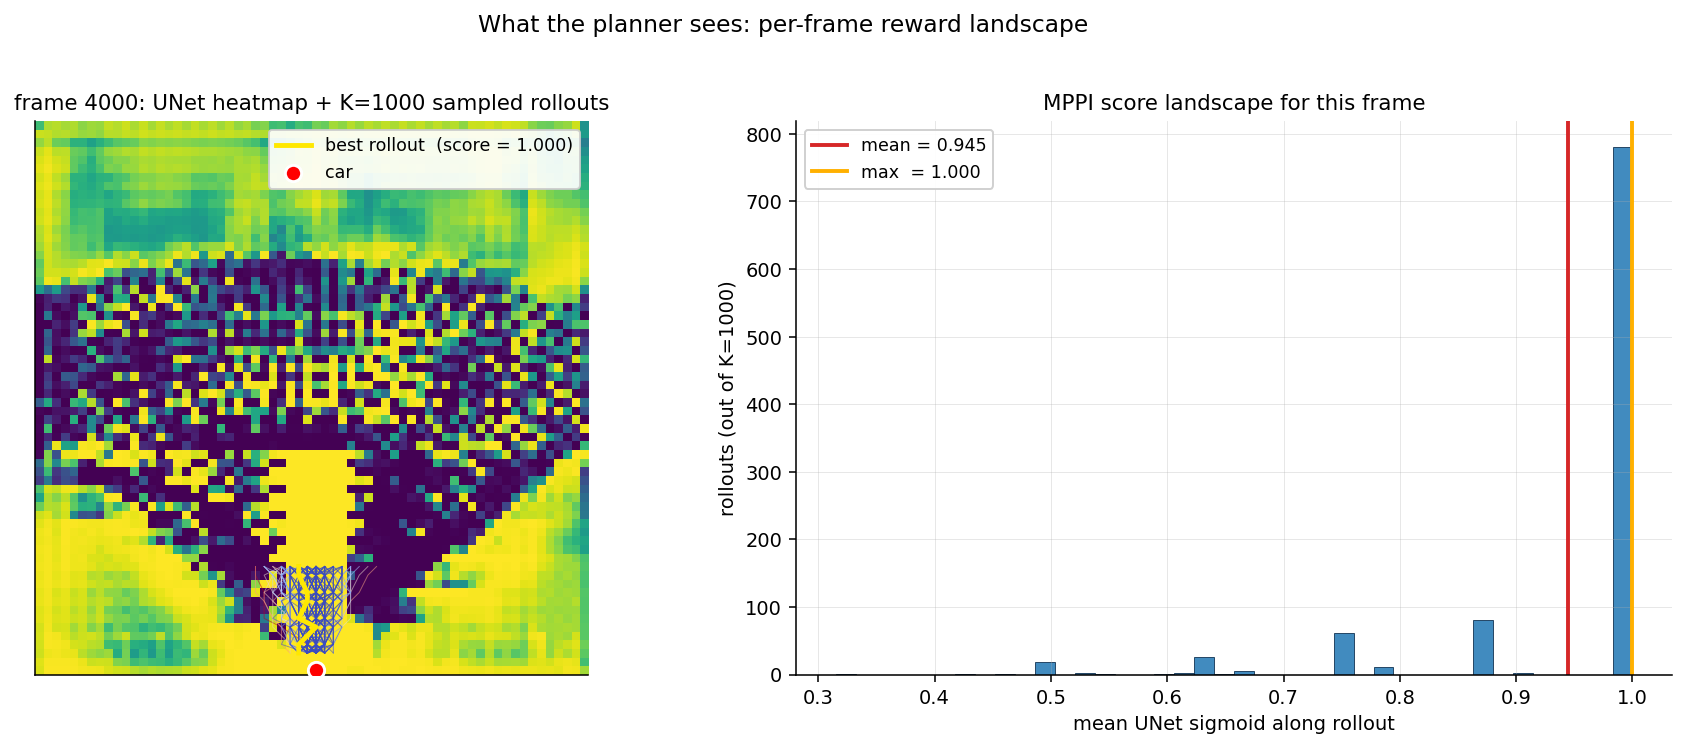
\includegraphics[width=\columnwidth]{../docs/plots/mppi_landscape.png}
  \caption{Per-frame planning landscape. Left: U-Net heatmap for frame
  $4000$ with K=1000 sampled MPPI rollouts overlaid (every fifth drawn for
  legibility). Right: histogram of the K rollout scores. Most rollouts
  cluster at $\sigm > 0.95$; the tail at lower scores represents trajectories
  that strayed into low-traversability regions.}
  \label{fig:mppi}
\end{figure}

%==============================================================================
\section{Visual diagnostic: perception vs.\ exploitation}
\label{sec:demo}

A full $8{,}331$-frame replay of the trained pipeline, including the
visualisations described below, is included with the project as
\texttt{demo.mp4} in the repository.

To separate the contribution of the learned reward from that of the
off-the-shelf planner, the demo overlays \emph{two} predicted paths on each
camera frame:

\begin{itemize}
  \item \textbf{Solid cyan line.} The MPPI committed path, computed by
        rolling out the post-update nominal sequence $\bar{U}$ from the car
        position. This is the trajectory the planner would execute on
        that frame.
  \item \textbf{Dashed white dots.} The U-Net greedy argmax path: for each
        forward row in the BEV grid, the column with maximum sigmoid
        within a local window of the previous row's argmax. This is the
        trajectory a greedy planner would steer toward if it trusted the
        reward signal alone.
\end{itemize}

\noindent
When the two paths coincide (most straight sidewalk segments), the
demonstration shows that the trained reward is \emph{usable} by a standard
sampling-based controller. When they diverge---typically on gradual
curves where the trained U-Net correctly tracks the curving sidewalk but
the MPPI nominal under-reacts---the demonstration shows that the
trained perception is correct and that the limitation lies with the
generic MPPI controller, not the perception. We discuss this further in
Section~\ref{sec:discussion}.

%==============================================================================
\section{Field testing status}
\label{sec:field}

The full hardware-integrated pipeline was verified on-bench: all $13$ ROS\,2
nodes launch via a single command (\texttt{drive.sh}), the ESC arms within
$5$\,s of launch via the retry-arming sequence, perception runs at the
target $5$\,FPS on the Jetson, and the safety-watchdog correctly enforces
the $500$\,ms command timeout. With the car held off the ground on a stand,
the steering servo physically tracks the predicted U-Net steering when
recorded sidewalk frames are played through the pipeline.

The planned closed-loop outdoor evaluation at the Sauls Ranch sidewalk
test loop was rained out during the booked weather window; the
NIR~\cite{creste} measurement reported by the original CREStE work
(NIR\,$= 0.05$ per $100$\,m on a 2\,km Mueller Lake Park loop) therefore
remains the headline limitation of this work.

To the extent that an offline diagnostic can substitute for a single short
closed-loop clip, we instead replay the trained pipeline across the
\emph{entire} training-set ($8{,}331$ frames; $\sim 4.6$ minutes at
$30$\,fps) so that per-frame perception and planning behaviour can be
audited by any reviewer; see \texttt{demo.mp4} and
Section~\ref{sec:demo}.

%==============================================================================
\section{Discussion and limitations}
\label{sec:discussion}

\paragraph{Training-set evaluation, not held-out.}
The training script does not maintain a train/val split; all $8{,}331$
frames are used for training. The margin of $+0.992$ should be read as
``the model fits its training labels nearly perfectly,'' not as
generalisation evidence. The two-path visual diagnostic provides our best
qualitative substitute pending the rained-out outdoor test.

\paragraph{Generic MPPI is the bottleneck.}
The committed MPPI path frequently under-reacts to gradual curvature. We
attribute this to three factors: (i) the score landscape under the trained
U-Net is flat on most frames (most rollouts score $\sigm > 0.95$), so
softmax-weighted averaging dilutes information; (ii) the $8$-step,
$1.8$\,m horizon cannot anticipate curves that begin more than two metres
ahead; and (iii) the controller has no explicit goal point when no GPS
waypoint is set. Replacing the sampling-based controller with a learned
policy that consumes the U-Net heatmap directly (e.g., behavioural cloning
on the same labels, or a small attention-based steering head) is the
obvious follow-up.

\paragraph{Monocular depth is the soft spot.}
Depth Anything V2 produces relative depth; our metric warp is a fixed
linear remap to $[0.5, 10]$\,m. This is correct on average across the
training set but produces systematic BEV distortion on extreme close-range
or far-field objects. A learned scale-recovery head would reduce the gap.

\paragraph{Online RLHF is wired but not exercised.}
The architecture includes an \texttt{intervention\_monitor\_node} that
detects mismatches between the planner output and human teleop input,
which could be used to drive an online BCE update on the U-Net from a
$M = 500$ FIFO replay buffer. We did not collect enough on-road
interventions to demonstrate this end-to-end and report it as future work.

%==============================================================================
\section{Conclusion}

CREStE-Nano demonstrates that the CREStE mapless-navigation paradigm can be
adapted to monocular RGB and \$500 of commodity hardware while retaining
the basic structure---BEV semantic features feeding a learned traversability
reward consumed by a sampling-based planner---and that the trained
perception generalises across an $8{,}331$-frame dataset of human
driving with negligible label-vs-prediction gap. Outdoor closed-loop
validation under the NIR metric of the original work remains the principal
open item.

%==============================================================================
\section*{Acknowledgements}

We thank Prof.\ Joydeep Biswas and the UT Austin Autonomous Mobile Robotics
Lab for the original CREStE work that this study extends, and the
maintainers of DINOv2 and Depth Anything V2 for releasing their checkpoints
publicly.

%==============================================================================
\bibliographystyle{IEEEtran}
\bibliography{references}

\end{document}
